\graphicspath{ {./img/TheFEM/} }
\chapter{Quadratures: numerical integration}

\section*{Preliminary}

The formulation of finite element algorithms is strongly based on the weak formulation of the boundary value problems. In loose terms, in typical finite element algorithms the boundary value problem originally written as a set of governing differential equations and properly specified boundary conditions, is re-formulated in the form of integral representations. For instance, this is the case in the boundary value problem of linearized theory of elasticity where the differential equations (corresponding to the equilibrium of a material point) and the tractions (and/or displacement) boundary conditions are shown to be equivalent to the the integral form representation of the principle of virtual displacements. In this case a finite element algorithm results from the discretization through interpolation schemes of the integrand appearing in the principle. However to generate an efficient method, valid over arbitrary domains it is necessary to implement effective numerical integration algorithms. To illustrate the need for numerical integration in the formulation of finite element methods consider a typical term resulting from the discretization of the internal virtual energy in the principle of virtual displacements such as the stiffness matrix given by: 



\begin{equation}
K^{QP} = \int_VH_{ij}^QC_{ijkl}H_{kl}^P\operatorname dV.
\label{sample integral 1}
\end{equation}

The accurate computation of these integrals is important to the formulation of the finite element algorithm. 

Note that the integration given by \eqref{sample integral 1} is conducted over a domain $V$ which is typically a finite element of arbitrary shape (e.g., a distorted quadrilateral element) therefore difficulting the computation of $K^{QP}$. This chapter discusses the most relevant details required in the numerical computation of integrals like the one appearing in \eqref{sample integral 1} which are typical in finite element algorithms. In the first part of the chapter we define a general formula for numerical integration. For completeness we derive integration formulas based on Lagrange interpolation although emphasis will be placed on the more efficient Gaussian integration formulas.

At the end of this chapter\footnote{{\bf This chapter, together with theoretical and computational learning activities is complemented by Jupyter Notebooks 5 and 6 available at the course REPO. Notebook 5 covers numerical integration as used in the finite element method, while notebook 6 combines interpolation theory with numerical integration in the calculation of the stiffness matrix for a finite element.}} the student should be able to:


\begin{itemize}
\item[•] Recognize the difference between explicit and numerical computation of integrals.
\item[•] Recognize the advantages and disadvantages of different numerical integration schemes.
\item[•] Propose integration schemes for specific finite elements.
\item[•] Implement efficient Python subroutines required in the integration of functions over specific finite elements.
\end{itemize}  



\section{Statement of the problem}

\begin{tcolorbox}
\paragraph*{A note on notation:}
Recall that in our indicial notation we are using subscripts to refer to the scalar components of a vector or a tensor function, while superscripts are reserved to represent elements of the interpolating polynomial. Thus for scalar components of a vector we use:

\[V_i\equiv\begin{bmatrix}V_x&V_y&V_z\end{bmatrix}.\]

For interpolation of a scalar function we use:

\[p(x)=L^Q(x)f^Q.\]

And for interpolation of a vector function we use:

\[u_i(x)=L_i^Q(x)u^Q\]

\end{tcolorbox}

In the most general case we are interested in numerically computing integrals of the general form


\begin{equation}
I\;=\iiint f(x,y,z)dV
\label{sample integral 2}
\end{equation}

where the triple integral represents an integration over a given volume. As in the case of interpolation theory, the problem of integration can also be solved from the fundamental problem of integrating a one-dimensional function like

\begin{equation}
\int\limits_a^b {f(x)dx}  \approx \sum\limits_{I = 1}^N {{w^I}} f({x^I}).
\label{quadra}
\end{equation}





In this fundamental one-dimensional problem the integral of a function $f(x)$ from $x = a$ to $x= b$ is approximated by a weighted summation of the values of the function at a set of $N$-points. In \eqref{quadra} $w^I$ represents a weighting factor associated to the value of the function $f({x^I})$ at the point $I$. 



This numerical approximation of the integral in terms of a weighted summation is called a quadrature formula and the derivation of a specific quadrature corresponds to prescribing the required number of points $N$, the corresponding weighting factors and the location of the $N$ sampling or integration points.

\paragraph*{Example}
Using the following set of quadrature points and weighting factors

\begin{center}
\begin{tabular}{cc}
  \hline
  $x^I$ & $w^I$ \\
  \hline
  $-0.86113$  & $0.34785$  \\
  $-0.33998$  & $0.65214$  \\
  $ +0.33998$  & $0.65214$  \\
  $ +0.86113$  & $0.34785$  \\
  \hline
\end{tabular}
%\captionof{table}{Definition of integration points and weighting factors for a numerical integration of the type $\int\limits_{ - 1}^{ + 1} {f(x)dx}$}
\label{ejemplo}
\end{center}

evaluate the integral


\begin{equation}
I = \int\limits_{ - 1}^{ + 1} {({x^3} + 4{x^2} - 10)dx}.
 \label{eqeje}
\end{equation} 


The numerical evaluation of the integral in \eqref{eqeje} just reduces to the computation of the following weighted summation:

\begin{align*}
\int\limits_{ - 1}^{ + 1} {({x^3} + 4{x^2} - 10)dx} \approx 0.34785 \cdot f( - 0.86113) + 0.65214 \cdot f( - 0.33998) \\
 + 0.34785 \cdot f(0.86113) + 0.65214 \cdot f(0.33998) = -17.3333
\end{align*}


\section{Numerical integration using interpolation polynomials}
A simple quadrature formula can be easily obtained if one represents the actual function $f(x)$ through a Lagrange based interpolation polynomial $p(x)$:


\begin{equation}
\int\limits_a^b {f(x)dx \approx \int\limits_a^b {p(x)dx} } .
 \label{polybased}
\end{equation} 

where


\begin{equation}
p(x) = {L^I}(x)f({x^I})
 \label{Lagracof}
\end{equation} 


and ${L^I}(x)$ is the Lagrange interpolation polynomial associated to point $x^I$.

Substituting \cref{Lagracof} in \cref{polybased} yields


\[\int\limits_a^b f(x)\ dx  \approx \int\limits_a^b L^I(x)f(x^I)dx  \equiv f(x^I)\int\limits_a^b L^I(x)dx\, \]

which can be written like

\begin{equation}
\int\limits_a^b {f(x)dx}  \approx \sum\limits_{I = 1}^N w^I f(x^I)
\label{general}
\end{equation}

after noticing that

\begin{equation}
w^I = \int\limits_a^b {L^I(x)\ dx}. 
\label{pesos}
\end{equation}

\begin{tcolorbox}
Integration schemes are classified in Newton-Cotes and Gaussian quadratures methods. In the first case the range of integration is divided into $N-1$ subintervals of constant size $\frac{b-a}{N-1}$ while in the second group one searches for the optimum location of the integration points inside the interval in order to obtain maximum accuracy. 
\end{tcolorbox}


\paragraph*{Example: Extended trapezoidal rule}
Consider the particular case in which $N=2$ (i.e., 1 integration interval). Clearly, in this case the size of the interval is $h=b-a$ and the interpolating polynomial is given by:

\[p(x) = {L^1}(x){f^1} + {L^2}(x){f^2} \equiv {L^1}(x)f(a) + {L^2}(x)f(b)\]

with interpolation polynomials corresponding to:

\[{L^1}(x) = \frac{{(x - {x^2})}}{{({x^1} - {x^2})}} \equiv  - \frac{1}{h}(x - b)\]

\[{L^2}(x) = \frac{{(x - {x^1})}}{{({x^2} - {x^1})}} \equiv \frac{1}{h}(x - a).\]

Substitution in \eqref{pesos} yields:

\[{w^1} =  - \frac{1}{h}\int\limits_a^b {(x - b)dx}  \equiv \frac{h}{2}\]

\[{w^2} =  + \frac{1}{h}\int\limits_a^b {(x - a)dx}  \equiv \frac{h}{2}\]

giving the final quadrature

\[I = {w^1}{f^1} + {w^2}{f^2} \equiv \frac{h}{2}\left[ {f(a) + f(b)} \right]\]

or equivalently:

\begin{equation}
\int\limits_a^b {f(x)dx = h\left[ {\frac{1}{2}{f(a)} + \frac{1}{2}{f(b)}} \right]}.
\label{trapecio}
\end{equation}

\paragraph*{Example: Computation of a definite integral}
Use the trapezoidal rule to compute the integral

\[I=\int\limits_{ - 1}^{ + 1} {({x^3} + 4{x^2} - 10)dx}.\]

In this case h=2.0, therefore:

\[I = f( - 1) + f( + 1) \equiv  - 7 - 5 =  - 12\]

\paragraph*{Example: Integration over two-dimensional domains.}
\Cref{fig:rieman} shows an schematic description of a two-dimensional domain (continuous black line) denoted by $R$. We wish to compute the integral



\[I = \iint\limits_R {f(x,y)dA}. \]

To proceed with the computation, the domain has been divided in $N$ rectagular subdomains (black dashed lines) in such a way that a typical subdomain has dimensions $\Delta {x_i} \times \Delta {y_i}$ as shown in the auxiliary figure.

\begin{figure}[H]
\centering
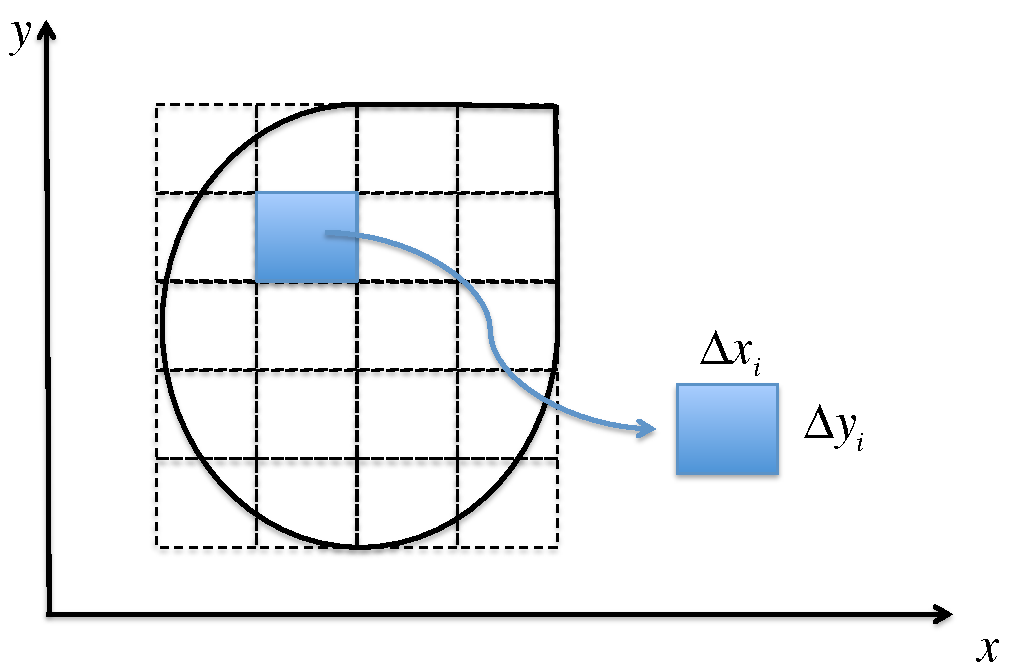
\includegraphics[width=10cm]{img/rieman.pdf}
\caption{Riemman partition for a two-dimensional domain.}
\label{fig:rieman}
\end{figure}

Defining

\[\left| p \right| = \max \left| {\Delta {x_i}} \right| \vee \max \left| {\Delta {y_i}} \right|\]

as the norm of the partition, we have, according to the definition of an integral as a Riemman sum that:


\[I = \iint\limits_R {f(x,y)dA}  \equiv \mathop {\lim }\limits_{\left| p \right| \to 0} \sum\limits_{j = 1}^N {f({x_j},{y_j})\Delta {x_j}} \Delta {y_j}.\]


Taking each one of the limits independently allows to identify 2 integration process such that the integral over $R$ reduces to the double integral given by:

\[I = \int {\int {f(x,y)dxdy} }. \]

To identify the integration limits consider \cref{fig:dirx} showing a rectangular integration domain with largest side parallel to the $x$ direction and with mid height corresponding to a $y$ constant value. The small sides of the rectangle have abscissas ${x_1}(y)$ and ${x_2}(y)$ respectively.


\begin{figure}[H]
\centering
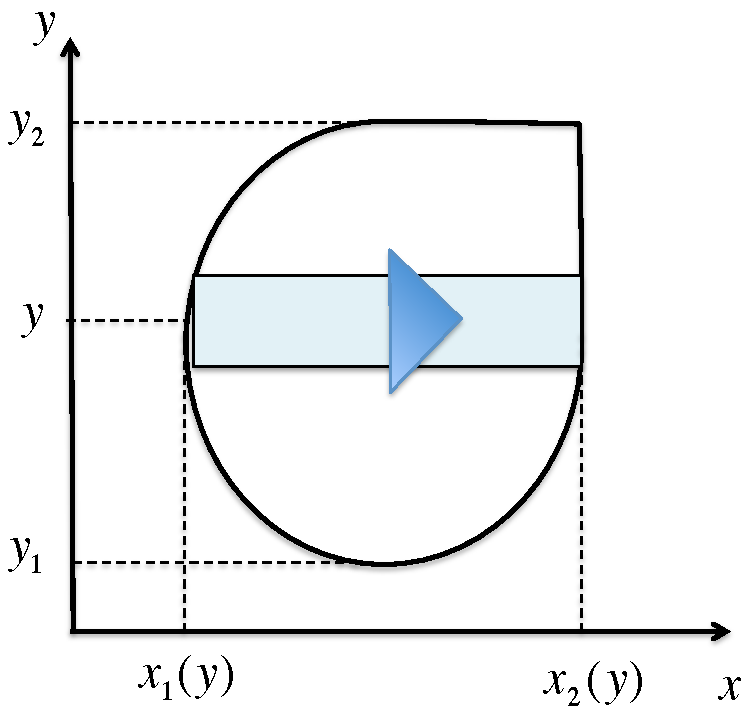
\includegraphics[width=10cm]{img/dirx.pdf}
\caption{Integration along the $x$ direction.}
\label{fig:dirx}
\end{figure}

Considering once again the definition of an integral as the limit of a Riemman sum we then have that for constant $y$ values the contribution to the integral over region $R$ of the rectangle bounded by ${x_1}(y)$ and ${x_2}(y)$ is given by:



\[\int\limits_{{x_1}(y)}^{{x_2}(y)} {f(x,y)dx}\]

in such a way that the computation of the integral over the full region $R$ is completed after repeating the process for constant values of $y$ varying between $y_1$ and $y_2$ giving for the total integral:


\begin{equation}
I = \int\limits_{{y_1}}^{{y_2}} {\left\{ {\int\limits_{{x_1}(y)}^{{x_2}(y)} {f(x,y)dx} } \right\}dy}
\label{iterada}
\end{equation}


To clarify  \cref{iterada}, note that the internal integral can be written as a function of $y$


\[F(y) = \int\limits_{{x_1}(y)}^{{x_2}(y)} {f(x,y)dx} \]

and the external integral like:


\[I = \int\limits_{{y_1}}^{{y_2}} {F(y)dy}. \]


Alternatively (see \cref{fig:diry}) it is possible to define:


\[H(x) = \int\limits_{{y_1}(x)}^{{y_2}(x)} {f(x,y)dy} \]

in such a way that the full integral $I$ is defined by:

\[I = \int\limits_{{x_1}}^{{x_2}} {H(x)dx}. \]

\begin{figure}[H]
\centering
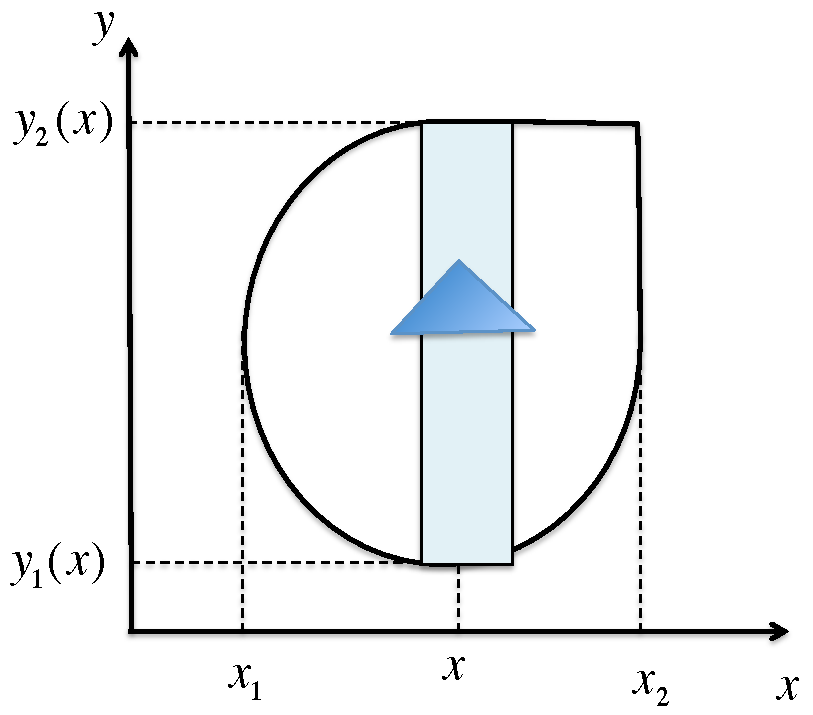
\includegraphics[width=10cm]{img/diry.pdf}
\caption{Integration along the $y$ direction.}
\label{fig:diry}
\end{figure}


Let us apply the previous ideas to compute the integral

\[I = \int {\int {x{y^2}} } dA\]

over the region shown in \cref{fig:ejeint}.



\begin{figure}[H]
\centering
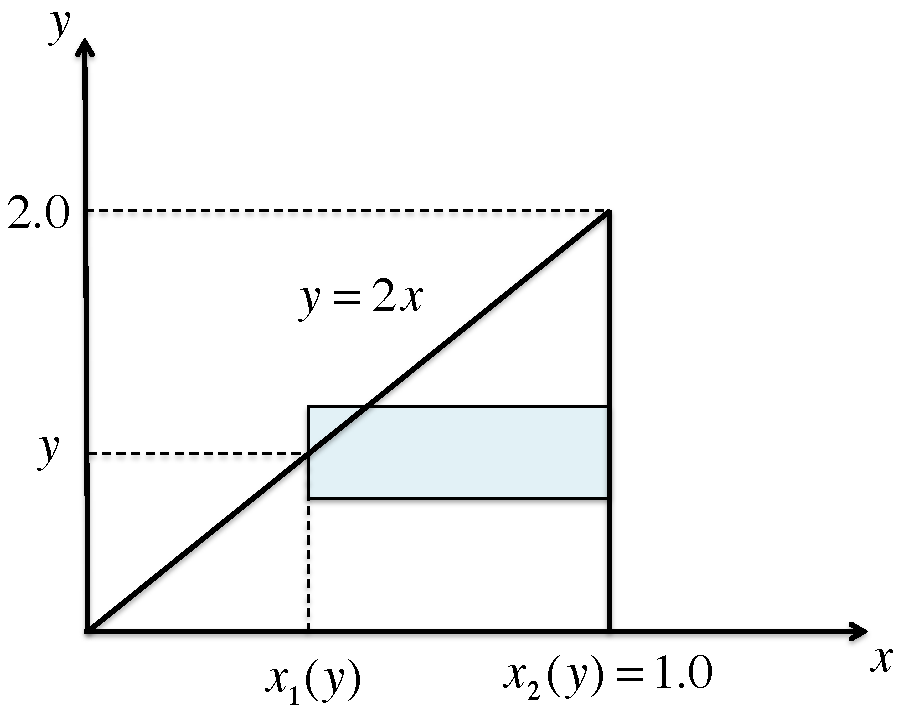
\includegraphics[width=10cm]{img/ejeint.pdf}
\caption{Integration along the $x$ direction over the triangular region $R$.}
\label{fig:ejeint}
\end{figure}

Identifying the lower and upper integration limits along the $y$ direction as ${y_1} = 0$ and ${y_2} = 2$ respectively, and the functions ${{x_1}(y)}$ and ${{x_2}(y)}$ like:

\[x_1(y) = \frac{y}{2}\]
and
\[x_2(y) = 1\]
we have that:
\[F(y) = \int\limits_{{x_1}(y)}^{1.0} {x{y^2}dx}  \equiv \int\limits_{y/2}^{1.0} {x{y^2}dx} \]

then

\[F(y) = \left. {\frac{1}{2}{x^2}{y^2}} \right|_{y/2}^{1.0} \equiv \frac{1}{2}{y^2} - \frac{1}{8}{y^4}\]

using this function to integrate in $y$ one finally gets that:

\[I = \int\limits_0^{2.0} {F(y)dy}  \equiv \int\limits_0^{2.0} {(\frac{1}{2}{y^2} - \frac{1}{8}{y^4})dy}  \equiv \frac{8}{{15}}.\]


Proceeding alternatively (see \cref{fig:ejeinty}) it is possible to write:

\[H(x) = \int\limits_{{y_1}(x)}^{{y_2}(x)} {x{y^2}dy} \]

and

\[I = \int\limits_{{x_1}}^{{x_2}} {H(x)dx} \]

\begin{figure}[H]
\centering
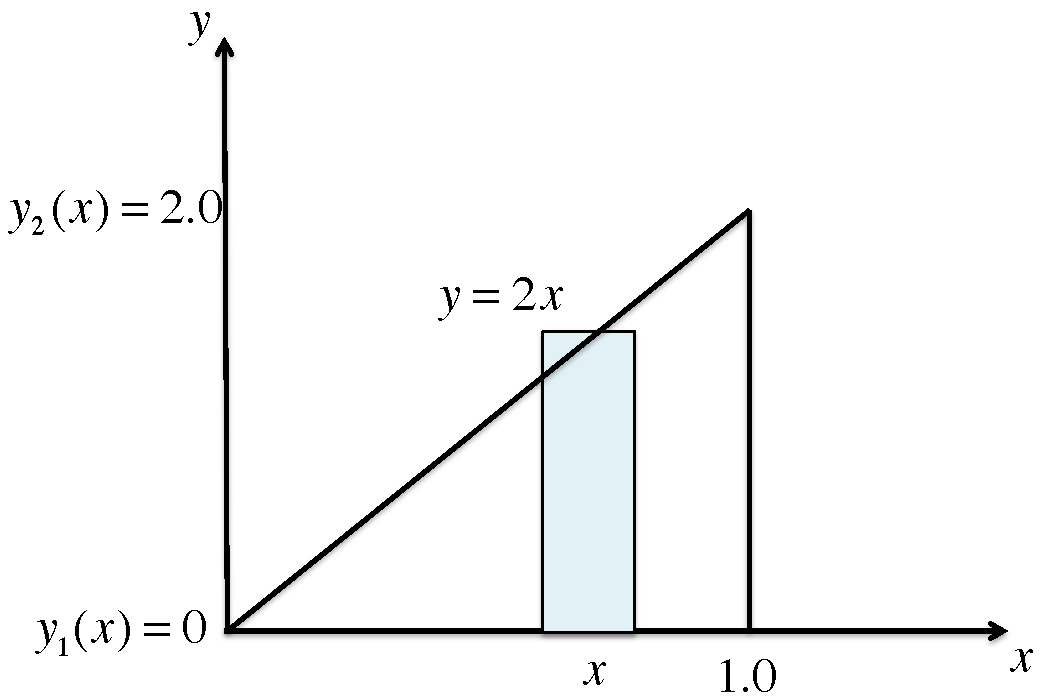
\includegraphics[width=10cm]{img/ejeinty.pdf}
\caption{Integration along the $y$ direction over the triangular region $R$.}
\label{fig:ejeinty}
\end{figure}

where:

\[{y_1}(x) = 0\]
\[{y_2}(x) = 2x\]

then

\[H(x) = \int\limits_0^{2x} {x{y^2}dy}  \equiv \left. {\frac{1}{3}x{y^3}} \right|_0^{2x} \equiv \frac{8}{3}{x^4}\]

so the integral reduces to:

\[I = \int\limits_0^{1.0} {\frac{8}{3}{x^4}dx}  \equiv \frac{8}{{15}}.\]

\section{Gaussian quadratures}
In the numerical quadrature corresponding to the extended trapezoidal rule written in the form

\begin{equation}
\int\limits_a^b {f(x)dx \approx \sum\limits_{I = 1}^{npts} {{w^I}f({x^I})} }
\label{quadra2}
\end{equation}

the integration points are equidistantly spaced. In a Gaussian quadrature in addition to adjusting the $N$ weighting factors $w^I$ one also leaves as adjustable parameters the location of the $N$ integration points. As a result, there are now $2N$ parameters to adjust in the derivation of an algorithm to numerically approximate the integral of $f(x)$ between $x=a$ and $x=b$ with the maximum accuracy and the minimum number of operations. This class of quadratures provide better precision than those based on Newton-Cotes techniques (such as the trapezoidal rule) when the function to integrate can be appropriately represented by a polynomial.

In general, different Gaussian quadratures are found in the literature reported in terms of tables providing the locations of integration (or Gauss) points and the corresponding weighting factors $w^I$. As an example \cref{ejemplo2} gives abscissas and weighting factors for a 4-point Gaussian quadrature.

\begin{center}
\begin{tabular}{cc}
  \hline
  $x^I$ & $w^I$ \\
  \hline 
  $-0.86113$  & $0.34785$  \\
  $-0.33998$  & $0.65214$  \\
  $ +0.33998$  & $0.65214$  \\
  $ +0.86113$  & $0.34785$  \\
  \hline
\end{tabular}
\captionof{table}{Abscissas and weighting factors to compute $\int\limits_{ - 1}^{ + 1} {f(x)dx}$}
\label{ejemplo2}
\end{center}

To facilitate coding of these quadratures and allow for approximation of general integrals, it is common to consider a primitive range of integration $[-1.0,+1.0]$ which requires transforming the original integral (including the function and its integration limits)to this primitive integral as discussed in \cref{isopar}. \Cref{fig:quagauss} schematizes the primitive integration range and the corresponding Gauss points denoted by the black $x$s. Transformation of a given integral to the primitive space is discussed at a later section.

\begin{figure}[H]
\centering
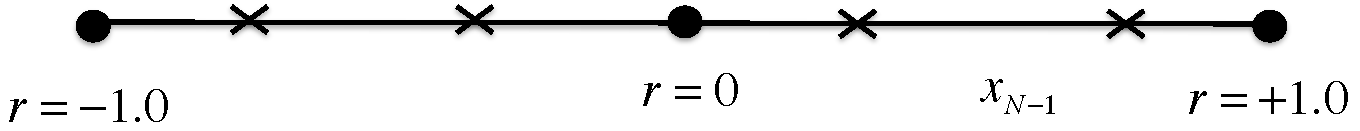
\includegraphics[width=10cm]{img/quagauss.pdf}
\caption{Schematic reperesentation of a Gaussian quadrature in the primitive range $[-1.0,1.0]$.}
\label{fig:quagauss}
\end{figure}

\paragraph*{Example:Derivation of a Gaussian quadrature}
Let $n=2$ and the integration interval $[a,b]=[-1,+1]$. Find $w^1$, $w^2$ and $x^1$, $x^2$ such the quadrature


\[I = \int\limits_{ - 1}^{ + 1} {f(x)dx}  \approx {w^1}f({x^1}) + {w^2}f({x^2})\]

integrated exactly the function  $f(x)$ corresponding to a third order polynomial like:



\[f(x) = {a_0} + {a_1}x + {a_2}{x^2} + {a_3}{x^3}.\]

Using $f(x)$ in $I$ and stating the integral for each term we have:


\[I = \int\limits_{ - 1}^{ + 1} {{a_0}dx}  + \int\limits_{ - 1}^{ + 1} {{a_1}xdx}  + \int\limits_{ - 1}^{ + 1} {{a_2}{x^2}dx}  + \int\limits_{ - 1}^{ + 1} {{a_3}{x^3}dx} \]

where:

\[\int\limits_{ - 1}^{ + 1} {dx}  = 2 = {w^1} \cdot 1 + {w^2} \cdot 1\]

\[\int\limits_{ - 1}^{ + 1} {xdx}  = 0 = {w^1} \cdot {x^1} + {w^2} \cdot {x^2}\]

\[\int\limits_{ - 1}^{ + 1} {{x^2}dx}  = \frac{2}{3} = {w^1} \cdot {({x^1})^2} + {w^2} \cdot {({x^2})^2}\]

\[\int\limits_{ - 1}^{ + 1} {{x^3}dx}  = 0 = {w^1} \cdot {({x^1})^3} + {w^2} \cdot {({x^2})^3}.\]

The resulting system of equations is solved in order to determine the 4 quadrature parameters, namely $w^1$, $w^2$ and $x^1$, $x^2$ giving $w^1 = 1$, $w^2 = 1$, $x^1 =  - \sqrt 3 /3$ and $x^1 =  + \sqrt 3 /3$ which allows us to write the quadrature in the general form:

\[I = \int\limits_{ - 1}^{ + 1} {f(x)dx}  \approx 1.0 \cdot f( - \sqrt 3 /3) + 1.0 \cdot f( + \sqrt 3 /3)\]

which is exact for polynomial functions of order at most 3.

The idea behind Gaussian quadratures can be extended to the integration of higher order polynomials, however its derivation requires an effective method to determine the weighting factors and the abscissas of the Gauss points. The next section discusses a method which is applicable to $2n$-order polynomials, in which advantage is taken from the property of orthogonality existing in certain special polynomials.




%\newpage
\section{Numerical integration in the finite element method}
\label{isopar}

\subsection{One-dimensional domains}
The systematization and construction of tables with coordinates and weighting factors for different quadratures is  useful if these are specified for a fixed range. For mathematical convenience it is common to use as base interval $[-1,+1]$. However considering that we are interested in integrating a function $f(x)$ in the general range with limits $x=a$ and $x=b$ it is required that we re-write the integral like:

\begin{equation}
\int\limits_a^b {f(x)dx \equiv } \int\limits_{ - 1}^{ + 1} {F(r)dr}. 
\label{trans}
\end{equation}

The mapping indicated in \cref{trans} is described in \cref{fig:map}, in which the space represented by the independent variable $x$ and contained between $x=a$ and $x=b$ is mapped to a fictitious "natural" space described by a new independent variable $r$ and enclosed in $r=-1$ y $r=1$.


\begin{figure}[H]
\centering
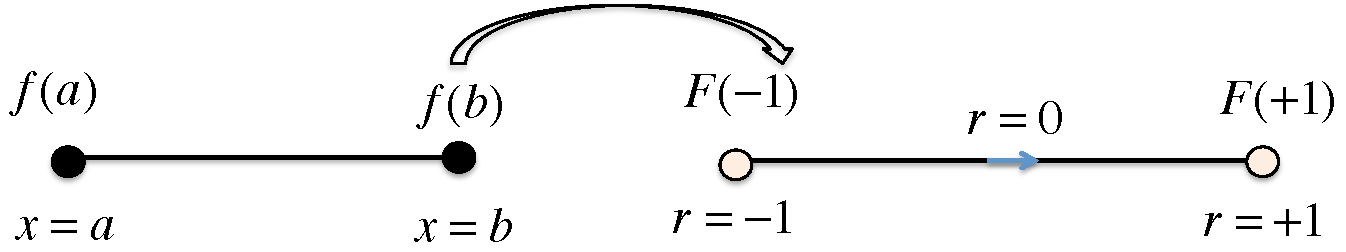
\includegraphics[width=12cm]{img/mapping.pdf}
\caption{Mapping between the physical space $[a,b]$ and the primitive or natural space $[-1.0,+1.0].$}
\label{fig:map}
\end{figure}

This is exactly the same transformation used when approximating unknown functions using interpolation theory over arbitrary distorted domains. Repeating for convenience, the transformation between both spaces can be written like:

\[x = x(r)\]
\[r = r(x)\]

and where $x(r)$ and $r(x)$ represent functional relationships between both spaces. For instance, in reference to \cref{fig:map}, it is evident that independent of the functional relationship this must satisfy the condition $x(-1.0)=a$ and $x(+1)=b$. Therefore, a valid relationship can be derived after assuming that both spaces are related through a Lagrange interpolating polynomials as follows:

\[x(r) = {L^1}(r)x({r^1}) + {L^2}(r)x({r^2})\]


and where the interpolation polynomials are given by:


\[{L^1}(r) = \frac{{(r - {r^2})}}{{({r^1} - {r^2})}} \equiv \frac{1}{2}(1 - r)\]

\[{L^2}(r) = \frac{{(r - {r^1})}}{{({r^2} - {r^1})}} \equiv \frac{1}{2}(1 + r)\]

which results in:

\[x(r) = \frac{1}{2}(a + b) + \frac{r}{2}(b - a).\]


It is also necessary to re-write $f(x)$ using as independent variable $r$ instead of $x$ using the functional relationship $x=x(r)$ like:

\[f = f(x) \equiv f[x(r)] = \hat F(r)\]

where $\hat F(r)$ represents the same function but now written in terms of $r$.


Finally, to complete the transformation it is necessary to transform physical differential space elements, that is $dx$. Proceeding directly from the mapping via the Lagrange interpolation polynomials we have:



\[\frac{{dx}}{{dr}} = \frac{{d{L^1}(r)}}{{dr}}x({r^1}) + \frac{{d{L^2}(r)}}{{dr}}x({r^2}) \equiv \frac{1}{2}(b - a)\]

and therefore

\[\frac{{dx}}{{dr}} = \frac{1}{2}(b - a)\]

which allows us to finally write the integral in the fictitious domain enclosed in $[-1, +1]$ according to:

\[\int\limits_a^b {f(x)dx \equiv } \int\limits_{ - 1}^{ + 1} {\hat F(r)\frac{\ell}{2}dr}  \equiv \int\limits_{ - 1}^{ + 1} {F(r)dr} \]


and where $\ell= \frac{1}{2}(b - a).$

\begin{tcolorbox}
The module {\bf Gaussutil()} in the finite element code {\bf SolidsPy} contains several one-dimensional and two-dimensional Gauss quadratures.
\end{tcolorbox}


\paragraph*{Example}


Use a 2 point Gaussian quadrature (see \cref{ejemplo3}) to evaluate the integral:

\[I = \int\limits_0^3 {({2^x} - x)dx}. \]


\begin{center}
\begin{tabular}{cc}
  \hline
  $x^I$ & $w^I$ \\
  \hline 
  $-0.577350269189626$  &  $1.000000$  \\
  $+0.577350269189626$  & $1.000000$  \\
  \hline
\end{tabular}
\captionof{table}{Abscissas and weighting factors to compute $\int\limits_{ - 1}^{ + 1} {f(r)dr}$}
\label{ejemplo3}
\end{center}

To perform the numerical integration using the 2-point Gaussian quadrature given in \cref{ejemplo3} it is necessary to transform the integration range and the integrand of the function to the range corresponding to $[-1.0,+1.0]$. The transformation is given by:

\[x(r) = \frac{3}{2} + \frac{3}{2}r\]

while the differential elements satisfy

\[dx = \frac{3}{2}dr.\]

To transform the function we use:

\[\hat f(r) = f[x(r)] \equiv f\left( {\frac{3}{2} + \frac{3}{2}r} \right)\]


from which:

\[I = \int\limits_0^3 {({2^x} - x)dx}  \equiv \int\limits_{ - 1.0}^{ + 1.0} {\left[ {{2^{\frac{3}{2}(1 + r)}} - \frac{3}{2}(1 + r)} \right]\frac{3}{2}dr} \]

and evaluating:

\[I = \sum\limits_{I = 1}^2 {{w^I}\left[ {{2^{\frac{3}{2}(1 + {r^I})}} - \frac{3}{2}(1 + {r^I})} \right]\frac{3}{2}}  = 1.0 \cdot (1.37678967978) + 1.0 \cdot (4.18374583924) \equiv 5.56053551\]

\subsection{Two-dimensional domains}
In the finite element method there is interest in computing integrals like:

\begin{equation}
I=\int_{V(\overrightarrow x)} f(\overrightarrow x)\operatorname dV(\overrightarrow x)
\label{integral}
\end{equation}

where $V(\overrightarrow x)$ is the domain of a typical finite element in a reference system with position vector $\overrightarrow x$. In one-dimensional problems $V(\overrightarrow x)\equiv\lbrack x_a,x_b\rbrack$; in two-dimensional problems $V(\overrightarrow x)$ is a plane surface; and in three-dimensional problems $V(\overrightarrow x)$ is a volume. Moreover, previously we have defined a finite element like a local interpolation space where values of a function are known at specific points (nodes). For instance, in two-dimensional space we had a quadrilateral bi-lineal element as the one shown in \cref{fig:generalElement}.

%
\begin{figure}[H]
\centering
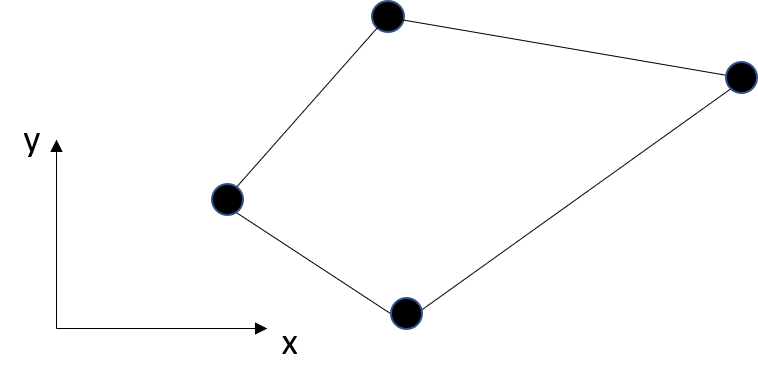
\includegraphics[width=8cm]{img/physical}
\caption{Arbitrary bi-lineal element defined in the physical space}
\label{fig:generalElement}
\end{figure}

As in the one-dimensional case discussed in the previous section, to conduct numerical integration in a systematic way, we actually need to transform generalized finite elements into canonical interpolation spaces (see \cref{fig:IsoTrans}).

\begin{figure}[H]
\centering
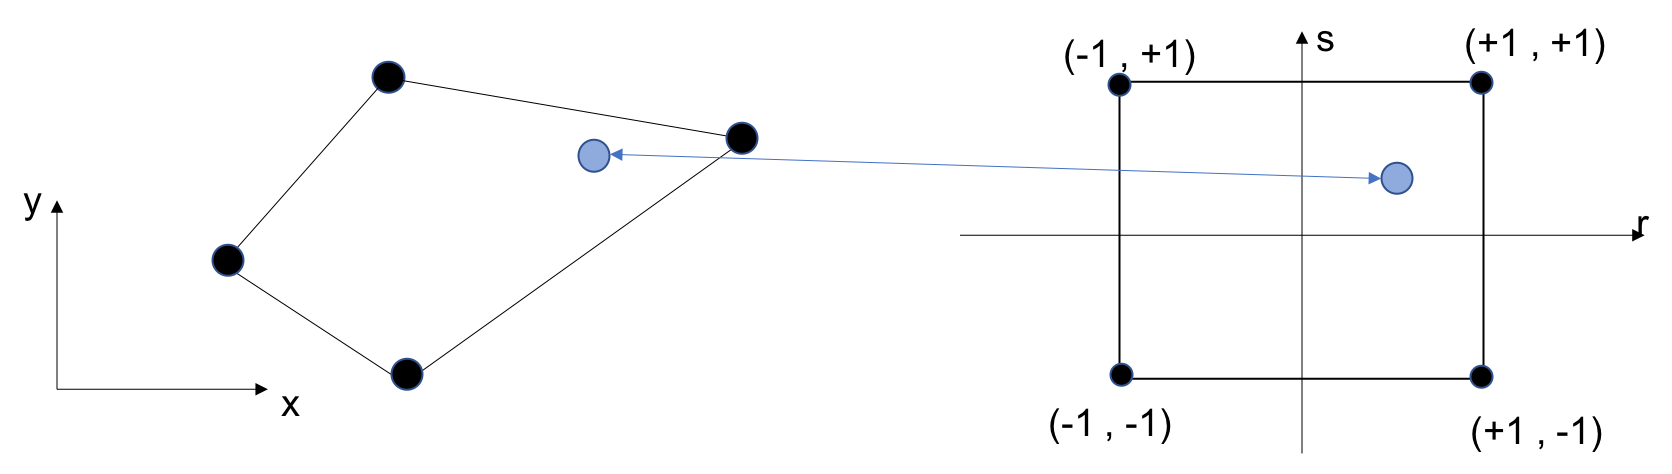
\includegraphics[width=12cm]{img/isopar}
\caption{Transformation from a general distorted element in the physical space to a perfect square in the natural space}
\label{fig:IsoTrans}
\end{figure}

Repeating the transformation for convenience, we have:

\begin{equation}
\begin{aligned}
x_i &=x_i(\overrightarrow r)\\
r_I &=r_I(\overrightarrow x)
\end{aligned}
\label{eq:transQ}
\end{equation}

where $\overrightarrow x$ and $\overrightarrow r$ denote position vectors in the physical and canonical space respectively. Using the above to transform functions we can write:



\begin{equation}
f=f(\overrightarrow x)\equiv f\lbrack x_i(\overrightarrow r)\rbrack\equiv F(\overrightarrow r).
\label{eq:FtransQ}
\end{equation}


\Cref{eq:FtransQ} above indicates that passing $f(\overrightarrow x)$ from the physical to the natural space representation corresponds to a change of variables. In the particular case of classical finite element methods the change of variables is conducted after approximating the physical geometry using interpolation. particularly, using the same set of shape functions as in the approximation of the primary fields we can write:

\begin{equation}
x_i(\overrightarrow r)=N_i^Q(\overrightarrow r)x^Q
\label{eq:Strans}
\end{equation}

where $x^Q$ denotes the spatial coordinates of nodal point $Q$ and $=N_i^Q(\overrightarrow r)$ is the shape function associated to the nodal point $Q$. According to this expression in the finite element method the geometry is interpolated in terms similar to the ones used for the primary field variable.

To transform the domain of integration we start once again from the general functional relationship:

\[x_i =x_i(\overrightarrow r)\]

and  use it to stablish the relationship between differential lengths in both spaces as:


\begin{equation}
dx_i=\frac{\partial x_i}{\partial r_J}dr_j.
\label{eq:diflen}
\end{equation}

The second order tensor $\frac{\partial x_i}{\partial r_J}$ appearing in \ref{eq:diflen} is the Jacobian of the transformation $J_{iJ}$ explicitly defined by;


\[J_{iJ}=\frac{\partial x_i}{\partial r_J}\]

and this tensor contains all the information regarding the geometric changes between both spaces. In terms of the shape functions it follows that:

\begin{equation}
J_{iJ}=\frac{\partial x_i}{\partial r_J}\equiv\frac{\partial N_i^Q}{\partial r_J}x^Q.
\label{eq:disJac}
\end{equation}

To complete the transformation we make use of Nanson's formula from continuum mechanics, from which:


\[ dV(\overrightarrow x)=\left|J\right|dV(\overrightarrow r)\]


where $\left|J\right|$ is the determinant of the Jacobian tensor. We can write for $I$ in both spaces:


\begin{equation}
I=\int_{V(\overrightarrow x)}f(\overrightarrow x)\operatorname dV(\overrightarrow x)\equiv\int_{V(\overrightarrow r)}F(\overrightarrow r)\left|J(\overrightarrow r)\right|\operatorname dV(\overrightarrow r)
\label{eq:twoInte}
\end{equation}


Consider now the particular case of a two-dimensional bi-lineal finite element discussed previously and its transformation into the natural space shown in \cref{fig:IsoMap}. Notice that this canonical element is a perfect square of element side $2.0$ contained between $x\in\left[-1.0\;,\;+1.0\right]$ and $y\in\left[-1.0\;,\;+1.0\right]$ which is the same range of the fundamental quadrature studied in the one-dimensional context.


\begin{figure}[H]
\centering
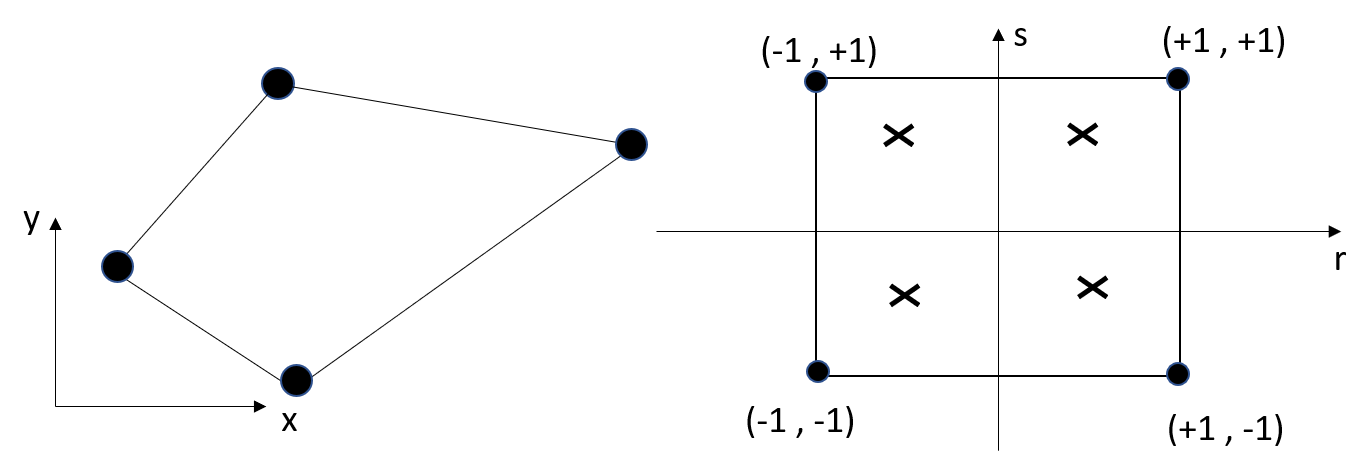
\includegraphics[width=12cm]{img/mapping2}
\caption{Transformation from a general distorted element in the physical space to a perfect square in the natural space}
\label{fig:IsoMap}
\end{figure}


In the particular case of the transformation described in \cref{fig:IsoMap} we have that


\[dV(\overrightarrow r)=drds\]

therefore

\[dV(\overrightarrow x)=\left|J\right|drds\]


and \cref{eq:twoInte} takes the form:


\begin{equation}
I=\int_{S(\overrightarrow x)}f(\overrightarrow x)\operatorname dS(\overrightarrow x)\equiv\int_{r=-1}^{r=+1}\int_{s=-1}^{s=+1}F(r,s)\left|J(r,s)\right|\operatorname drds.
\label{eq:bilineal}
\end{equation}

To integrate \ref{eq:bilineal} using a quadrature of $Ngpts$ integration points we use:

\begin{equation}
I=\int_{r=-1}^{r=+1}\int_{s=-1}^{s=+1}F(r,s)\left|J(r,s)\right|\operatorname drds\approx\sum_{i=1}^{Ngpts}\sum_{j=1}^{Ngpts}F(r_i,s_j)\left|J(r_i,s_j)\right|w_iw_j
\label{eq:Iquad}
\end{equation}

which can be simplified into

\begin{equation}
I=\int_{r=-1}^{r=+1}\int_{s=-1}^{s=+1}F(r,s)\left|J(r,s)\right|\operatorname drds\approx\sum_{k=1}^{Ngpts\ast Ngpts}F(r_k,s_k)\left|J(r_k,s_k)\right|\alpha_k
\label{eq:Iquad1}
\end{equation}

which the one-dimensional version resulting from the iterated summation. The points marked with a cross in \cref{fig:IsoMap} represent integration points.

\begin{tcolorbox}
Notebook 5 in the REPO uses transformation or mapping from the physical to the canonical space, together with numerical integration, to compute the area of a distorted quadrilateral finite element.
\end{tcolorbox}



\subsection{Matrix formulation}
For the computer implementation of the different methods discussed so far it is practical to use a combined notation in terms of index and matrix representation of variables. Consider the interpolated version of a vector field, for instance the displacement vector in elasticity:

\begin{equation}
u_i(\overrightarrow r)=N_i^Q(\overrightarrow r)u^Q
\label{eq:mixed}
\end{equation}


in which:

\begin{itemize}
\item[•] Susbcript $i$ refers to the normal components of vectors in the physical space
\item[•] Superscript $Q$ refers to the contribution from nodal point $Q$ to the approximated field (in this case $u_i(\overrightarrow r)$)
\item[•] $\overrightarrow r$ position vector of a point in the natural space. In index notation we refer to the scalar components of this vector using capitalized subscripts as $\overrightarrow r=r_I$
\item[•] $N_i^Q(\overrightarrow r)$ shape function associated to the nodal point $Q$ evaluated at the point $\overrightarrow r$.
\end{itemize}

The contribution to the $Q$ nodal point implicit in \cref{eq:mixed} can be written in explicit expanded form as:
\[
\begin{array}{l}\begin{Bmatrix}u\\v\end{Bmatrix}=\left[\cdots\begin{array}{cc}N^Q(\overrightarrow r)&0\\0&N^Q(\overrightarrow r)\end{array}\cdots\right]\begin{Bmatrix}\vdots\\\begin{array}{c}u^Q\\v^Q\end{array}\\\vdots\end{Bmatrix}.\\\end{array}
\]


To compute the Jacobian tensor at point $\overrightarrow r$ assume that the nodal coordinates are stored in a matrix



\[
\begin{array}{l}coord\;=\begin{bmatrix}\vdots\\\begin{array}{cc}x^Q&y^Q\end{array}\\\vdots\end{bmatrix}\\\end{array}
\]

then we can further express:

\begin{equation}
\begin{array}{l}\begin{bmatrix}\frac{\partial x}{\partial r}&\frac{\partial y}{\partial r}\\\frac{\partial x}{\partial s}&\frac{\partial y}{\partial s}\end{bmatrix}=\begin{bmatrix}\cdots&\begin{array}{c}\frac{\partial N^Q}{\partial r}\\\frac{\partial N^Q}{\partial s}\end{array}&\cdots\end{bmatrix}\begin{bmatrix}\vdots\\\begin{array}{cc}x^Q&y^Q\end{array}\\\vdots\end{bmatrix}\\\end{array}
\label{eq:jac}
\end{equation}

Having found the Jacobian of the transformation the remaining step consists in transforming the integrand $f(\overrightarrow{x})$. This step however is not constructed explicitly  but it depends on the structure of $f(\overrightarrow{x})$. In most finite element algorithms the problem formulation involves spatial derivatives of the primary function rather than the primary function itself. To consider these terms in the transformed version of $I$, it becomes necessary to relate spatial differentiation in both spaces. To clarify this aspect of the formulation assume that $I$ is of the form:

\[I=\int_{V(\overrightarrow x)}\frac{\partial f}{\partial\overrightarrow x}\operatorname dV(\overrightarrow x).\]

We already found that

\[\operatorname dV(\overrightarrow x)=\left|J\right|\operatorname dV(\overrightarrow r)\]

and to transform the integrand


\[\frac{\partial f}{\partial\overrightarrow x}\]

we recall that in the finite element method the interpolation of the primary variable is conducted directly in the natural space. This means that we already have $F(\overrightarrow r)$ or more explicitly that:





\[F(\overrightarrow r)=N^Q(\overrightarrow r)F^Q.\]

However to capture correctly the physics of the problem we are interested in finding

\[\frac{\partial f}{\partial\overrightarrow x}.\]

Using implicit differentiation:

\[\frac{\partial f}{\partial x_i}=\frac{\partial F}{\partial r_J}\frac{\partial r_J}{\partial x_i}\]

and re-arranging for convenience we write

\begin{equation}
\frac{\partial f}{\partial x_i}=\frac{\displaystyle\partial r_J}{\displaystyle\partial x_i}\frac{\partial F}{\partial r_J}.
\end{equation}

Notice that the first factor is the Jacobian inverse given by;

\[\frac{\partial r_J}{\partial x_i}=\left(J_{iJ}\right)^{-1}\equiv\left(\frac{\displaystyle\partial x_i}{\displaystyle\partial r_J}\right)^{-1}\]

while the second factor reads:

\[\frac{\partial F}{\partial r_J}=\frac{\partial N^Q}{\partial r_J}F^Q\]

which allows us to write:

\[I=\int_{V(\overrightarrow x)}\frac{\partial f}{\partial\overrightarrow x}\operatorname d{V(\overrightarrow x)}\equiv\int_{V(\overrightarrow r)}J_{iJ}^{-1}\frac{\displaystyle\partial N^Q}{\displaystyle\partial r_J}\left|J(\overrightarrow r)\right|\operatorname dV(\overrightarrow r).\]


\begin{tcolorbox}
As an in-class activity Notebook 6 in the REPO requires the computation of the stiffness matrix for a plane strain solid element.
\end{tcolorbox}

\paragraph*{Proposed problems}
\begin{enumerate}

\item \label{punto01} Compute the integral of the function

\[f(x,y)=4x^2+3xy+y^2\]

over the two-dimensional domains shown in the figure

\begin{figure}[H]
\centering
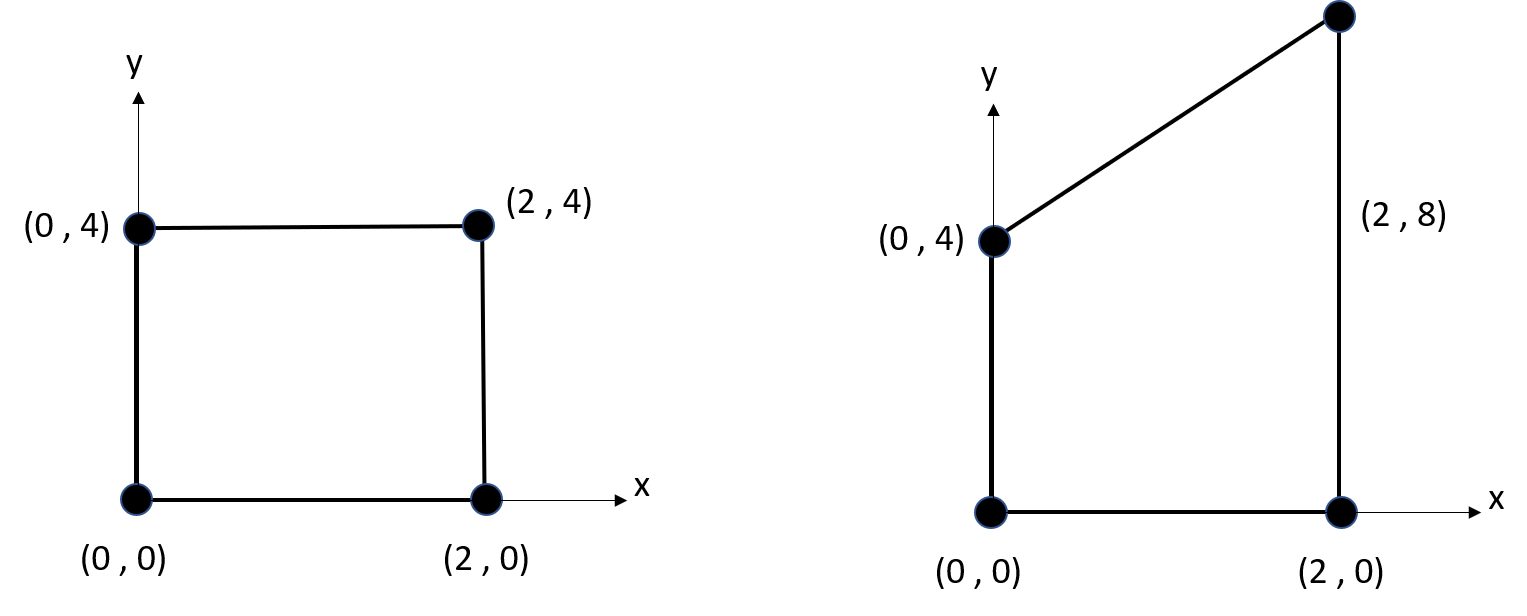
\includegraphics[width=12cm]{domain1}
\caption{Integration domains for problem 1}
\label{fig:intdomains}
\end{figure}

\item \label{punto02} Compute the jacobian of the transformation of the domains shown in the figure

\begin{figure}[H]
\centering
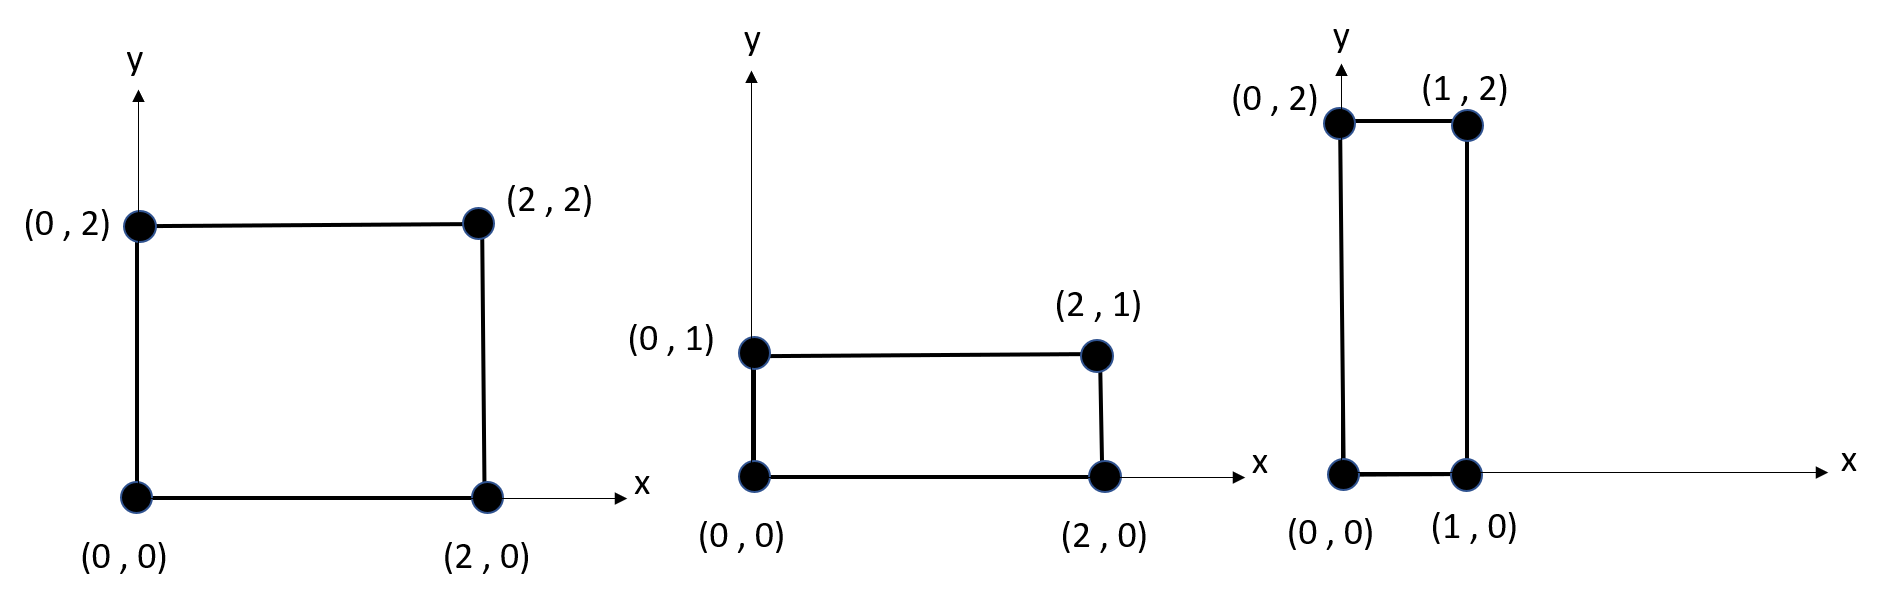
\includegraphics[width=14cm]{domain2}
\caption{Integration domains for problem 1}
\label{fig:jacdomains}
\end{figure}

to a perfectly square canonical element of side $2.0$.

\item \label{punto03} Compute the integral of the function

\[f(r,s)=rs\]

over the triangular domain shown in the figure

\begin{figure}[H]
\centering
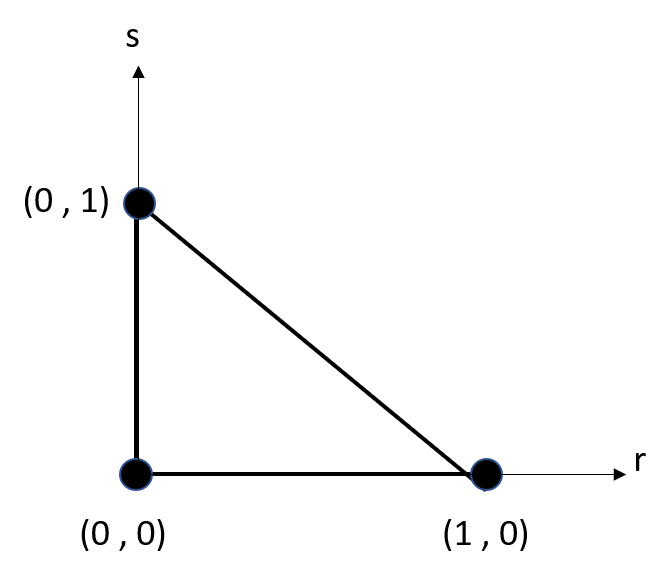
\includegraphics[width=7cm]{domain3}
\caption{Integration domains for problem 1}
\label{fig:tridomains}
\end{figure}



\end{enumerate}
